% Cubit panel 4-Layer architecture -- CONCEPT diagram (TikZ blocks + arrows + grouping).
% Recipe: radia_mcp.figure  figure_diagram_recipes(topic="concept_diagram").
% Build:  pdflatex panel_4layer_architecture.tex
\documentclass[tikz,border=2mm]{standalone}
\usepackage{newtxtext,newtxmath}
\usetikzlibrary{positioning, fit, backgrounds, arrows.meta}
\begin{document}
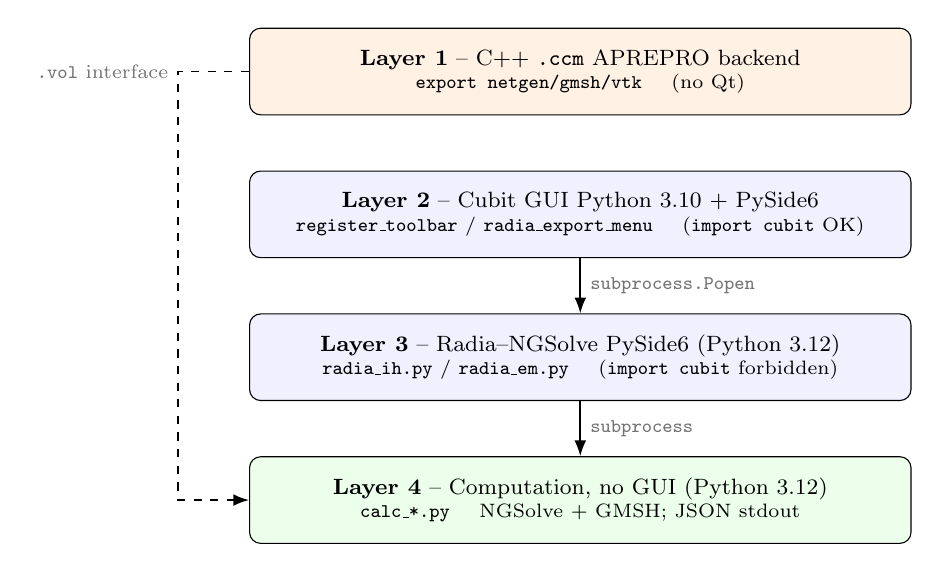
\begin{tikzpicture}[font=\footnotesize, >={Latex[length=2mm]},
  layer/.style={rectangle, draw, rounded corners, minimum width=84mm, minimum height=11mm,
                align=center, fill=black!4},
  flow/.style={-{Latex[length=2mm]}, semithick},
  note/.style={font=\scriptsize, text=black!55},
]
  \node[layer, fill=orange!10] (l1)
    {\textbf{Layer 1} -- C++ \texttt{.ccm} APREPRO backend\\[-1pt]
     {\scriptsize \texttt{export netgen/gmsh/vtk} \quad (no Qt)}};
  \node[layer, fill=blue!6, below=7mm of l1] (l2)
    {\textbf{Layer 2} -- Cubit GUI Python 3.10 + PySide6\\[-1pt]
     {\scriptsize \texttt{register\_toolbar} / \texttt{radia\_export\_menu} \quad (\texttt{import cubit} OK)}};
  \node[layer, fill=blue!6, below=7mm of l2] (l3)
    {\textbf{Layer 3} -- Radia--NGSolve PySide6 (Python 3.12)\\[-1pt]
     {\scriptsize \texttt{radia\_ih.py} / \texttt{radia\_em.py} \quad (\texttt{import cubit} forbidden)}};
  \node[layer, fill=green!8, below=7mm of l3] (l4)
    {\textbf{Layer 4} -- Computation, no GUI (Python 3.12)\\[-1pt]
     {\scriptsize \texttt{calc\_*.py} \quad NGSolve + GMSH; JSON stdout}};
  \draw[flow] (l2) -- node[right, note]{\texttt{subprocess.Popen}} (l3);
  \draw[flow] (l3) -- node[right, note]{\texttt{subprocess}} (l4);
  % .vol = the sole Cubit <-> NGSolve interface (produced by L1, consumed by L4)
  \draw[flow, dashed] (l1.west) -- ++(-9mm,0)
        node[left, note]{\texttt{.vol} interface} |- (l4.west);
\end{tikzpicture}
\end{document}
